\documentclass[11pt,a4paper]{article}

% ------------------------------------------------------------------
% Packages (same style as the project log and the analysis report)
% ------------------------------------------------------------------
\usepackage[T1]{fontenc}
\usepackage[utf8]{inputenc}
\usepackage{lmodern}
\usepackage[margin=2.5cm]{geometry}
\usepackage{booktabs}
\usepackage{tabularx}
\usepackage{array}
\usepackage{longtable}
\usepackage{xcolor}
\usepackage{enumitem}
\usepackage{fancyhdr}
\usepackage{titlesec}
\usepackage{listings}
\usepackage{graphicx}
\usepackage{amsmath}
\usepackage{caption}
\usepackage{hyperref}

\hypersetup{colorlinks=true, linkcolor=blue!50!black, urlcolor=blue!50!black}

\definecolor{codebg}{gray}{0.96}
\definecolor{okgreen}{RGB}{0,120,60}
\definecolor{warnorange}{RGB}{200,110,0}

\lstset{
  basicstyle=\ttfamily\small,
  backgroundcolor=\color{codebg},
  frame=single,
  rulecolor=\color{gray!40},
  breaklines=true,
  columns=fullflexible,
  keepspaces=true,
  showstringspaces=false
}

\newcommand{\code}[1]{\texttt{#1}}
\newcommand{\pass}{\textcolor{okgreen}{\textbf{PASS}}}
\newcolumntype{Y}{>{\raggedright\arraybackslash}X}
\newcolumntype{R}{>{\raggedleft\arraybackslash}X}

\setlength{\emergencystretch}{3em}
\setlength{\parskip}{4pt}
\setlength{\parindent}{0pt}

\pagestyle{fancy}
\fancyhf{}
\lhead{\small TeraNova -- FPGA Acceleration}
\rhead{\small Simulation report -- K.~Janssen (4994817)}
\cfoot{\small\thepage}
\renewcommand{\headrulewidth}{0.4pt}

\titleformat{\subsection}{\normalfont\large\bfseries}{\thesubsection}{1em}{}

% ------------------------------------------------------------------
\begin{document}

\begin{titlepage}
\centering
\vspace*{3cm}
{\LARGE\bfseries Simulation Report\par}
\vspace{0.5cm}
{\Large Functional and Cycle-Level Simulation of the\\FPGA Matrix-Multiplication Accelerator\par}
\vspace{0.3cm}
{\large TeraNova -- FPGA Acceleration\par}
\vspace{2cm}
\begin{tabular}{@{}ll@{}}
\textbf{Author}          & Kai Janssen \\
\textbf{Student number}  & 4994817 \\
\textbf{Date}            & 29 October 2026 \\
\textbf{Platform}        & AMD ZCU102 (Zynq UltraScale+ \code{xczu9eg-ffvb1156-2-e}) \\
\textbf{Tools}           & GHDL 4.1.0; Vitis HLS 2025.1.1 (C simulation, C/RTL co-simulation) \\
\end{tabular}
\vfill
{\small All results in this report come from simulation. None of them has been measured on the board yet.\par}
\end{titlepage}

\begin{abstract}
\noindent
While the ZCU102 board is not available, I simulated every part of the accelerator that can be simulated without it. This covers the complete programmable-logic (PL) data path, from the block RAMs to the result memory, including the real RTL that Vitis HLS generated for \code{RAM\_INTERFACE}. All 96 simulation runs produce the correct $50\times50$ result: 94 GHDL runs (two data sets, a range of writer speeds and memory latencies, a restart without reset, three partitioner versions) and the two Vitis HLS simulations from 7 October. With realistic memory behaviour, one multiplication takes \textbf{101\,186 clock cycles (1.012\,ms at 100\,MHz)} on the PL. Handshake monitors confirm the main finding of the earlier analysis with exact numbers. The partitioner hands over one block pair every 101 cycles, and 50 of those cycles are wait states that do no work. The multiplier is busy only 5\,000 of 101\,008 cycles (4.95\,\%). The simulation also found one thing the analysis had not: the generated \code{RAM\_INTERFACE} waits for the write response after every 5-element burst. In steady state it needs $85 + 5L$ cycles per output block, where $L$ is the memory's write-response latency. That is harmless today, but it becomes the bottleneck once the partitioner is made faster. I simulated two faster partitioners as the first improvement. Removing the wait states halves the PL run time to 51\,186 cycles. A pipelined version that reads one element per cycle brings it to \textbf{27\,186 cycles (0.272\,ms, 3.7$\times$ faster)}. That version only reaches its speed if the memory confirms a write within 37 cycles; above that, the result writer sets the pace. The CPU side (loading the matrices and reading the result back) cannot be simulated and is left for the board measurement.
\end{abstract}

\setcounter{tocdepth}{1}
\tableofcontents
\newpage

% ==================================================================
\section{What can be simulated, and what cannot}
% ==================================================================
Table~\ref{tab:scope} lists each part of the system and whether simulation can give a reliable answer for it. The rule is simple: anything inside the PL is described by VHDL or HLS code that can be simulated cycle by cycle. The ARM processor, the PS--PL interconnect and the DDR4 controller are not, so their timing has to be measured on the board.

\begin{table}[h]
\centering
\begin{tabularx}{\textwidth}{@{}>{\raggedright\arraybackslash}p{5.2cm}Y>{\raggedright\arraybackslash}p{3.6cm}@{}}
\toprule
\textbf{Part} & \textbf{How} & \textbf{Simulated?} \\
\midrule
\code{matrix\_partitioner\_B} (rev.~4) & Its VHDL, in GHDL & Yes, cycle-exact \\
\code{MatMul5x5\_PAR\_IF} (multiplier) & Its VHDL, in GHDL & Yes, cycle-exact \\
\code{MatMul5x5\_Accumulator} & Its VHDL, in GHDL & Yes, cycle-exact \\
\code{RAM\_INTERFACE} (result writer) & HLS C simulation; xsim co-simulation; generated RTL in GHDL & Yes, cycle-exact \\
Result memory (PL DDR4 via MIG) & AXI4 memory model with adjustable latency & Behaviour only; latency is a parameter \\
Block RAMs (\code{Part0}--\code{Part3}) & Behavioural model, read latency 1 & Yes (as configured in the design) \\
CPU loading A and B (10\,000 AXI writes) & -- & No: needs the board \\
CPU reading the result (2\,500 AXI reads) & -- & No: needs the board \\
Interrupt path \code{done} $\rightarrow$ GIC & -- & No: needs the board \\
Timing closure at 100\,MHz & -- & No: needs the licensed Vivado build \\
\bottomrule
\end{tabularx}
\caption{Simulation scope.}
\label{tab:scope}
\end{table}

% ==================================================================
\section{Simulation setup}
% ==================================================================

\subsection{Testbenches}
Most of the testbenches already existed from the IP restoration in October. For this report I added a performance version of the chain testbench and a version that uses the real HLS RTL. The design files themselves were not changed.

\begin{table}[h]
\centering
\begin{tabularx}{\textwidth}{@{}lYl@{}}
\toprule
\textbf{Testbench} & \textbf{What it does} & \textbf{Status} \\
\midrule
\code{RAM\_INTERFACE\_TEST.cpp} & HLS C testbench: feeds 2 complete matrices block by block, checks every word in memory and the \code{done} behaviour & Existing (2 Oct) \\
\code{tb\_chain.vhd} + \code{run.py} & Complete PL data path with a model of the writer handshake; compares the $50\times50$ result with Python & Existing (2 Oct) \\
\code{tb\_chain\_perf.vhd} + \code{run\_perf.py} & Same as \code{tb\_chain}, plus passive monitors on every valid/ready handshake that count cycles per stage & New \\
\code{tb\_chain\_rtl.vhd} + \code{run\_rtl.py} & Data path with the \emph{real} \code{RAM\_INTERFACE} RTL from Vitis HLS, writing through \code{m\_axi} into an AXI4 memory model; ends when \code{done} rises. \code{RUNS=2}: a second complete run without reset (restart test) & New \\
\code{axi\_mem\_model.vhd} & AXI4 write slave: up to 4 outstanding addresses, byte strobes, write response \code{B\_LATENCY} cycles after \code{WLAST}, optional throttling of \code{WREADY}; counts bursts and beats & New \\
\code{run\_all.py} & Compiles everything and runs the 31 GHDL cases for the current design; writes \code{results.json} & New \\
\code{run\_variants.py} & Runs the testbenches for each partitioner version (rev.~4, v5a, v5b) in its own build folder (63 runs); writes \code{variants\_results.json} & New \\
\bottomrule
\end{tabularx}
\caption{Testbenches used in this report (all in \code{C:\textbackslash PLD\textbackslash sim}, HLS in \code{C:\textbackslash PLD\textbackslash hls\textbackslash RAM\_INTERFACE}).}
\end{table}

The monitors in \code{tb\_chain\_perf} only read signals; they do not drive anything. This means the cycle counts are those of the unmodified design. Every testbench run also checks the complete result against a reference computed in Python, so a performance number is only reported for a run that produced the correct result.

\subsection{Test data}
Two data sets are used:
\begin{itemize}[noitemsep]
  \item \textbf{\code{helloworld} data:} $A_{ij} = 50i + j + 1$, $B_{ij} = 50i + j + 2$, the same values as the board application;
  \item \textbf{random 64-bit data:} full-range random values (fixed seed). This checks the upper bits, the wrap-around modulo $2^{64}$ and the signed/unsigned mismatch noted as finding F9 in the analysis.
\end{itemize}

\subsection{Clock and units}
All PL logic runs on one 100\,MHz clock in the design, so one cycle is 10\,ns. Cycle counts start at the start pulse.

\subsection{The generated RTL in GHDL}
\code{tb\_chain\_rtl} uses the seven VHDL files that Vitis HLS generated on 7 October (\code{work\textbackslash hls\textbackslash impl\textbackslash vhdl}), i.e.\ exactly the RTL inside the packaged IP. GHDL needed one change: line 539 of \code{RAM\_INTERFACE\_gmem\_m\_axi.vhd} uses a VHDL-2019 conditional constant, which GHDL's VHDL-2008 mode does not accept. In the simulation copy (\code{sim\textbackslash hls\_rtl}) that line is replaced by an equivalent function call, marked \code{SIM PATCH}. It selects the same value. The packaged IP is not affected.

% ==================================================================
\section{Functional results}
% ==================================================================
All simulation runs of the current design produce the correct result (Table~\ref{tab:func}). The HLS C simulation, synthesis and xsim co-simulation are from 7 October (logs in \code{hls\textbackslash RAM\_INTERFACE}); all GHDL runs were done today from a clean folder with \code{run\_all.py} and \code{run\_variants.py}. The partitioner versions of Section~\ref{sec:variants} pass the same tests.

\begin{table}[h]
\centering
\begin{tabularx}{\textwidth}{@{}YYr@{}}
\toprule
\textbf{Test} & \textbf{Condition} & \textbf{Result} \\
\midrule
HLS C simulation, \code{RAM\_INTERFACE} & 2 matrices back to back, full 64-bit values & \pass \\
HLS C synthesis + packaging & \code{xczu9eg}, 100\,MHz target & \pass \\
C/RTL co-simulation (xsim, \code{ap\_ctrl\_hs} variant) & 2 $\times$ 100 blocks & \pass \\
\code{tb\_chain}, writer model & \code{helloworld} data and random 64-bit data & \pass{} (2 runs) \\
\code{tb\_chain}, slow writer & 1\,500 cycles per block, both data sets & \pass{} (2 runs) \\
\code{tb\_chain\_perf} & both data sets & \pass{} (2 runs) \\
\code{tb\_chain\_perf}, writer sweep & 30 to 1\,500 cycles per block (11 points) & \pass{} (11 runs) \\
\code{tb\_chain\_rtl}, real \code{RAM\_INTERFACE} & both data sets, $L = 20$ cycles & \pass{} (2 runs) \\
\code{tb\_chain\_rtl}, latency sweep & $L$ = 1 to 500 cycles (10 points) & \pass{} (10 runs) \\
\code{tb\_chain\_rtl}, throttled write channel & \code{WREADY} low every 2nd / 4th cycle & \pass{} (2 runs) \\
\code{tb\_chain\_rtl}, restart & second complete run without reset, both data sets & \pass{} (2 runs) \\
\bottomrule
\end{tabularx}
\caption{Functional results. ``PASS'' means all 2\,500 result values are correct and, for \code{tb\_chain\_rtl}, no AXI protocol assertion fired and \code{done} rose before the time-out.}
\label{tab:func}
\end{table}

Three behaviours that matter for the board run are confirmed:
\begin{itemize}[noitemsep]
  \item \textbf{No lost or duplicated blocks under back-pressure.} Even when the writer is 50\,\% slower than the data path, all 100 output blocks arrive exactly once. This was the weakness of the previous group's \code{ap\_none} handshake (finding F11).
  \item \textbf{\code{done} rises only after the last write is acknowledged.} In \code{tb\_chain\_rtl} it rises 179 cycles after the last block was accepted ($L = 20$), after the AXI write response of the final burst.
  \item \textbf{Restart works without a reset.} In \code{tb\_chain\_rtl} with \code{RUNS=2}, a second start after \code{done} gives a second correct result in exactly the same time (101\,186 cycles); \code{done} goes low during the second run and rises again at its end. The HLS testbench and co-simulation show the same for the writer alone. This is what the board application relies on when it runs 10 times in a row.
\end{itemize}

% ==================================================================
\section{Where the clock cycles go}
% ==================================================================

\subsection{Per-stage counters}
Table~\ref{tab:perf} shows the monitor results of \code{tb\_chain\_perf}. They are identical for both data sets: the run time does not depend on the values.

\begin{table}[h]
\centering
\begin{tabularx}{\textwidth}{@{}Yrl@{}}
\toprule
\textbf{Measurement} & \textbf{Value} & \textbf{Meaning} \\
\midrule
Total PL run time & 101\,008 cycles & 1.010\,ms at 100\,MHz \\
Block pairs handed to the multiplier & 1\,000 & $10 \times 10 \times 10$ \\
Interval between block pairs & 101 cycles (min = max) & partitioner sets the pace \\
Cycles the partitioner waited for the multiplier & 0 & the multiplier never blocks \\
Multiplier busy (not ready) & 5\,000 cycles & 4.95\,\% of the run \\
Multiplier latency per block pair & 5 cycles (min = max) & accept $\rightarrow$ product valid \\
Cycles the multiplier waited for the accumulator & 0 & \\
Output blocks to the writer & 100 & \\
Interval between output blocks & 1\,010 cycles & $10 \times 101$ \\
First output block & cycle 1\,018 & \\
Cycles the accumulator waited for the writer & 0 & with a 30-cycle writer model \\
\bottomrule
\end{tabularx}
\caption{Handshake monitor results, \code{tb\_chain\_perf}, writer model busy 30 cycles per block.}
\label{tab:perf}
\end{table}

The total follows exactly from the partitioner's state machine:
\begin{equation*}
T_\text{PL} = \underbrace{1000}_{\text{block pairs}} \times \big(\underbrace{25 \times 4}_{\text{elements} \times \text{states}} + \underbrace{1}_{\text{handshake}}\big) + \underbrace{2}_{\text{start}} + \underbrace{5}_{\text{multiplier}} + \underbrace{1}_{\text{accumulator}} = 101\,008 \text{ cycles}
\end{equation*}
The 4 states per element are \code{ISSUE\_ADDR}, \code{WAIT1}, \code{WAIT2} and \code{CAPTURE}. The last three terms are the latency of the final block: start-pulse detection, the multiply, and the last accumulation.

\begin{figure}[h]
\centering
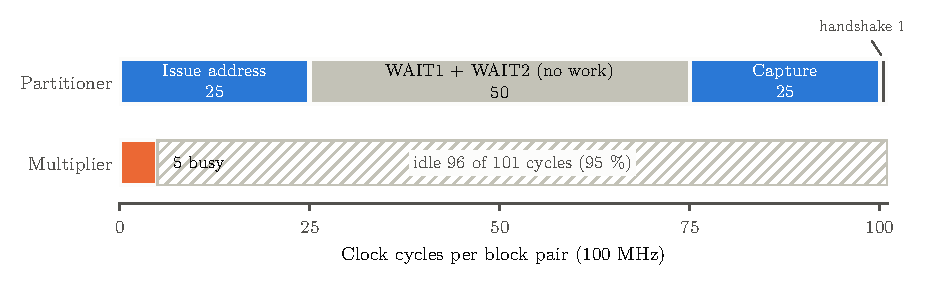
\includegraphics[width=\textwidth]{figures/cycle_budget.pdf}
\caption{One block pair takes 101 cycles. Half of them are the \code{WAIT1}/\code{WAIT2} states, and the multiplier works for only 5.}
\label{fig:budget}
\end{figure}

\subsection{What this confirms}
Figure~\ref{fig:budget} turns three estimates from the analysis report into measured facts:
\begin{itemize}[noitemsep]
  \item \textbf{F3, unnecessary wait states:} 50 of every 101 cycles (49.5\,\%) are spent in \code{WAIT1}/\code{WAIT2}. The BRAMs in the design (and the model) have a read latency of 1 cycle, so the data is valid one cycle after the address and the two wait states add nothing. Section~\ref{sec:variants} simulates versions without them.
  \item \textbf{F4, one element per cycle at best:} even without wait states, the 25 elements of a block are read one at a time.
  \item \textbf{F7, oversized multiplier:} the single-cycle $5\times5$ multiplier, which uses 1\,257 DSPs, is idle 95\,\% of the time. The analysis estimated $\sim$5 cycles per block pair and $\sim$95\,\% idle; the simulation measures exactly 5 and 95.05\,\%.
\end{itemize}

% ==================================================================
\section{The real result writer}
% ==================================================================

\subsection{Run time with the generated RTL}
With the real \code{RAM\_INTERFACE} RTL and a write-response latency of $L = 20$ cycles, the complete PL run, from start until \code{done}, takes \textbf{101\,186 cycles (1.012\,ms)}. The data path itself is unchanged: all counters of Table~\ref{tab:perf} are identical. The rest is the writer finishing the last block: \code{done} rises $79 + 5L$ cycles after the writer accepted it.

\begin{table}[h]
\centering
\begin{tabularx}{\textwidth}{@{}Yrl@{}}
\toprule
\textbf{Measurement} & \textbf{Value} & \textbf{Note} \\
\midrule
Start $\rightarrow$ \code{done} & 101\,186 cycles & 1.012\,ms at 100\,MHz \\
Last block accepted $\rightarrow$ \code{done} & $79 + 5L$ cycles & 179 cycles at $L = 20$ \\
AXI write bursts & 504 & 500 rows + 4 splits \\
AXI write beats & 2\,500 & one per result value \\
Burst length & 1 to 5 beats & one row of a $5\times5$ block \\
Write bursts in flight (max) & 2 & the IP is configured for 4 \\
AXI read transactions & 0 & as intended \\
\bottomrule
\end{tabularx}
\caption{\code{tb\_chain\_rtl}: real \code{RAM\_INTERFACE} RTL, AXI memory model with $L = 20$.}
\label{tab:rtl}
\end{table}

\textbf{Short bursts (finding F6).} The writer forms one burst per row of a block: 5 consecutive addresses. The next row of the same block is 50 elements further on in memory, so it needs a new burst. The 4 extra bursts appear where a row crosses a 4\,KB address boundary: the result is 20\,000 bytes, so it crosses the boundaries at 4, 8, 12 and 16\,KB, and AXI does not allow a burst across them. The \code{max\_write\_burst\_length=16} setting is never reached.

\textbf{A wait after every row.} The writer's time per block grows by 5 cycles for every extra cycle of memory latency (Figure~\ref{fig:sweep}b). The reason is in the generated pipeline (\code{RAM\_INTERFACE\_RAM\_INTERFACE\_Pipeline\_ROWS\_COLS.vhd}). Vitis HLS put the wait for the write response (\code{m\_axi\_gmem\_0\_BVALID}) inside the pipelined loop, at the end of every row. So the writer stalls 5 times per block, once for each burst, instead of letting the responses overlap. For a fast memory this costs 79 cycles per block. The xsim co-simulation of 7 October measured 780\,ns, i.e.\ 78 cycles, per block, which is consistent. It also explains why the HLS estimate of 41 cycles was too low: HLS schedules with an ideal memory.

\subsection{When does the writer become the bottleneck?}
The accumulator presents a finished block every 1\,010 cycles. As long as the writer needs less than that, it is hidden behind the partitioner. Figure~\ref{fig:sweep} shows both ways this was tested. In (a), the writer model is given a fixed busy time per block; in (b), the real RTL runs against memories with increasing write-response latency. The two agree: the run time stays at the partitioner limit until the writer needs more than about 1\,009 cycles per block. The real RTL keeps up at $L = 185$ and stalls the accumulator from $L = 186$ (1.86\,\textmu s). In steady state it needs $85 + 5L$ cycles per block: $79 + 5L$ to write a block, plus 6 cycles to finish the call and accept the next block. This simple rule predicts the limit exactly for all three partitioner versions (Section~\ref{sec:variants}). Above the limit, every extra cycle of latency adds 500 cycles to the run (100 blocks $\times$ 5 rows).

\begin{figure}[h]
\centering
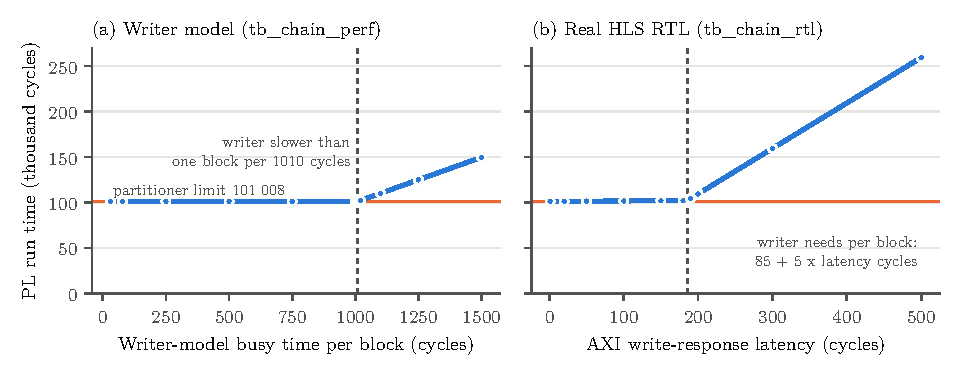
\includegraphics[width=\textwidth]{figures/bottleneck_sweep.pdf}
\caption{PL run time against writer speed. (a) Writer model with a fixed busy time per block. (b) Real \code{RAM\_INTERFACE} RTL against the AXI memory's write-response latency. The orange line is the partitioner limit (101\,008 cycles).}
\label{fig:sweep}
\end{figure}

Throttling the write channel has little effect. With \code{WREADY} low every 2nd or 4th cycle, the run takes 101\,211 or 101\,194 cycles (+25 and +8). Data beats are not the limit; waiting for write responses is.

\subsection{What it means for the board}
The latency of the PL DDR4 path (SmartConnect, clock-domain crossing to the 300\,MHz MIG, the DDR4 itself) is not known yet. It is very unlikely to be anywhere near 1.86\,\textmu s, so with today's partitioner the real writer should not slow the run down. The predicted PL compute time on the board is therefore 1.011\,ms ($L = 1$) to 1.013\,ms ($L = 50$).

% ==================================================================
\section{HLS synthesis results}
% ==================================================================
For completeness, the synthesis results of the rebuilt \code{RAM\_INTERFACE} (Vitis HLS 2025.1.1, 7 October, \code{work\textbackslash hls\textbackslash syn\textbackslash report\textbackslash RAM\_INTERFACE\_csynth.rpt}):

\begin{table}[h]
\centering
\begin{tabularx}{\textwidth}{@{}YR@{}}
\toprule
\textbf{Item} & \textbf{Result} \\
\midrule
Estimated clock period (target 10\,ns) & 7.30\,ns ($F_\text{max} \approx 137$\,MHz) \\
Main loop \code{ROWS\_COLS} & pipelined, II = 1, depth 11 \\
Latency per block (HLS estimate, ideal memory) & 41 cycles \\
Latency per block (co-simulation, xsim) & 78 cycles \\
Latency per block (GHDL, $L = 1$) & 79 cycles \\
Resources & 2\,708 FF, 1\,943 LUT, 2 DSP, 0 BRAM ($<$1\,\%) \\
\bottomrule
\end{tabularx}
\caption{HLS results of \code{RAM\_INTERFACE}.}
\end{table}

% ==================================================================
\section{Prediction for the board baseline}
% ==================================================================
Simulation fixes the PL part of the baseline. The end-to-end time on the board is
\begin{equation*}
T_\text{total} \;=\; \underbrace{10\,000 \cdot t_\text{write}}_{\text{load A, B}} \;+\; \underbrace{T_\text{PL}}_{\approx\,1.012\text{ ms (simulated)}} \;+\; \underbrace{2\,500 \cdot t_\text{read}}_{\text{read back C}}
\end{equation*}
Here $t_\text{write}$ and $t_\text{read}$ are the times of one CPU access across the PS--PL boundary. The measurement application in \code{C:\textbackslash PLD\textbackslash baseline} measures both directly (its ``latency probes''). Table~\ref{tab:predict} lists what simulation predicts and what the board has to add.

\begin{table}[h]
\centering
\begin{tabularx}{\textwidth}{@{}YYY@{}}
\toprule
\textbf{Quantity} & \textbf{Simulation} & \textbf{Board} \\
\midrule
PL compute (start $\rightarrow$ \code{done}) & 1\,011--1\,013\,\textmu s ($L \le 50$) & to measure; should match \\
Load A and B (10\,000 writes) & not simulatable & to measure \\
Read-back (2\,500 reads) & not simulatable & to measure \\
CPU-only reference & not simulatable & to measure \\
Correct result, restart & PASS (2 runs without reset) & to confirm with 10 runs \\
\code{done} interrupt & not simulatable & to confirm \\
\bottomrule
\end{tabularx}
\caption{Simulation prediction and the remaining board measurements.}
\label{tab:predict}
\end{table}

If the board's PL compute time differs from 1.011--1.013\,ms by more than a few microseconds, the hardware does not behave like the simulated RTL. That would point at the build (for example a stale bitstream) rather than the design.

% ==================================================================
\section{Simulated first improvement: a faster partitioner}\label{sec:variants}
% ==================================================================
The analysis report names the partitioner's wait states as the cheapest improvement. I wrote two versions and ran them through exactly the same testbenches as the current design. Both keep the entity name, generics, ports, block order and output packing of revision~4, so they are drop-in replacements (\code{sim\textbackslash variants}):
\begin{itemize}[noitemsep]
  \item \textbf{v5a, without wait states:} revision~4 with \code{WAIT1} and \code{WAIT2} removed; nothing else changed. 2 cycles per element.
  \item \textbf{v5b, pipelined:} a new BRAM address every cycle; each element is captured two clock edges after its address was set (address register, then the BRAM's read latency of 1). 1 cycle per element plus 2 to drain the pipeline.
\end{itemize}

Both rely on the BRAM read latency being exactly 1 cycle and the address multipliers adding no delay. I checked this in the block design's IP configuration (\code{.xci} files of \code{Part0}--\code{Part3} and \code{mult\_gen\_0/1}): all four BRAMs have \code{C\_READ\_LATENCY\_B = 1} with no output registers, and both multipliers have \code{C\_LATENCY = 0}. The testbench's BRAM model therefore matches the hardware.

\subsection{Results}
\begin{table}[h]
\centering
\begin{tabularx}{\textwidth}{@{}Yrrr@{}}
\toprule
 & \textbf{rev.~4 (current)} & \textbf{v5a} & \textbf{v5b} \\
\midrule
Cycles per block pair & 101 & 51 & 27 \\
Output block every & 1\,010 cycles & 510 cycles & 270 cycles \\
PL run, writer model (\code{tb\_chain\_perf}) & 101\,008 & 51\,008 & 27\,008 \\
PL run, real \code{RAM\_INTERFACE}, $L = 20$ & 101\,186 & 51\,186 & 27\,186 \\
\quad at 100\,MHz & 1.012\,ms & 0.512\,ms & 0.272\,ms \\
\quad speed-up of the PL part & 1.00$\times$ & 1.98$\times$ & 3.72$\times$ \\
Multiplier busy & 4.95\,\% & 9.80\,\% & 18.51\,\% \\
Largest $L$ the writer can hide (simulated) & 185 cycles & 85 cycles & 37 cycles \\
Functional tests (both data sets, back-pressure, restart) & \pass & \pass & \pass \\
\bottomrule
\end{tabularx}
\caption{The three partitioner versions in the same testbenches (\code{run\_variants.py}). Cycle counts are identical for \code{helloworld} and random 64-bit data.}
\label{tab:variants}
\end{table}

Table~\ref{tab:variants} shows that both versions do exactly what was expected. The run time follows the cycles per block pair: v5a halves it and v5b takes 27\,186 cycles. That is 3.72$\times$ faster on the PL side and close to the $\sim$4$\times$ the analysis estimated. All functional tests pass for both versions: both data sets, a writer that is 50\,\% slower than the data path (back-pressure), and a second run without reset.

\begin{figure}[h]
\centering
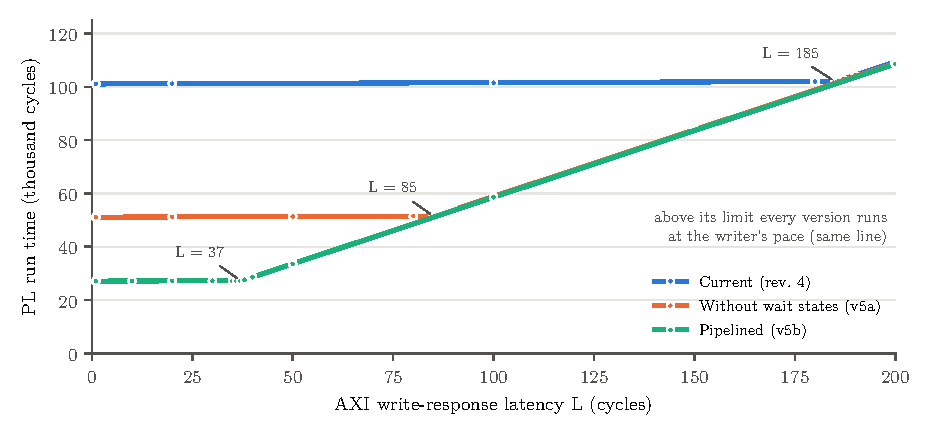
\includegraphics[width=\textwidth]{figures/variants_latency.pdf}
\caption{PL run time of the three partitioner versions against the write-response latency of the result memory (real \code{RAM\_INTERFACE} RTL). Each version is flat until the writer can no longer keep up; above that point all versions run at the writer's pace.}
\label{fig:variants}
\end{figure}

\subsection{The writer becomes the limit}
Figure~\ref{fig:variants} confirms the prediction of Section~5.2. A faster partitioner delivers finished blocks more often, so the writer has less time for each. With v5b it gets 270 cycles per block, so it can only hide a write-response latency of up to 37 cycles (370\,ns at 100\,MHz); from 38 cycles on it stalls the accumulator. Above its limit each version runs on the same line: the writer, not the partitioner, then sets the speed, and a faster partitioner gains nothing.

A latency of a few hundred nanoseconds is within the range a DDR4 path through a SmartConnect and a clock-domain crossing can have. Whether v5b reaches its full 3.7$\times$ on the board therefore depends on a latency that is not measured yet. Two follow-ups make it independent of that latency:
\begin{itemize}[noitemsep]
  \item change \code{RAM\_INTERFACE} so that it no longer waits for each row's write response before the next row (overlapping responses), or collect a full result row and write it as one long burst;
  \item check the result in \code{tb\_chain\_rtl}: the writer's limit should move far to the right in Figure~\ref{fig:variants}.
\end{itemize}

\subsection{What is needed to build it}
\begin{enumerate}[noitemsep]
  \item Copy \code{sim\textbackslash variants\textbackslash matrix\_partitioner\_B\_v5b.vhd} over the partitioner source in \code{ip\_repo\textbackslash}\allowbreak\code{matrix\_partitioner\_B} (keep the old file in \code{backup}).
  \item Re-package it with core revision 5 (copy of \code{1\_repackage\_partitioner.tcl}) and upgrade it in the block design; the ports are unchanged, so no rewiring is needed.
  \item Badr builds the bitstream. Timing at 100\,MHz should be checked: v5b computes a new address every cycle with the same address arithmetic that revision~4 already uses.
  \item Run the measurement application on the board and compare the PL compute time with 0.272\,ms.
\end{enumerate}
I recommend building v5b rather than v5a. It costs the same build effort and gives almost twice the gain of v5a.

% ==================================================================
\section{Limitations}
% ==================================================================
\begin{itemize}[noitemsep]
  \item The AXI memory model is ideal apart from its fixed write-response latency. The real path has a SmartConnect, a clock-domain crossing and DDR4 refresh, so its latency varies.
  \item The BRAM model reproduces the configured read latency of 1 cycle, not the Xilinx BRAM primitive itself.
  \item The address multipliers (\code{mult\_gen}, constant $\times4$) are not in the testbench; the partitioner addresses the BRAM model directly. They have latency 0 in the design (checked in their \code{.xci} files), so they add no cycles.
  \item Nothing here covers timing closure; that needs the licensed implementation run.
\end{itemize}

% ==================================================================
\section{Conclusion}
% ==================================================================
Every part of the PL data path was simulated and gives the correct $50\times50$ result in all 96 simulation runs, including with the real HLS-generated result writer, under heavy back-pressure and after a restart without reset. One multiplication takes 101\,186 cycles, or 1.012\,ms at 100\,MHz, and this is the PL compute time the board measurement should reproduce. The handshake monitors show exactly where that time goes: the partitioner needs 101 cycles per block pair, half of them wait states, while the multiplier works 5 of those cycles. The simulation also exposed a limit in the generated \code{RAM\_INTERFACE}, a write-response wait after every row. It costs nothing today. For the first improvement I simulated two faster partitioners; the pipelined one (v5b) brings the PL run to 27\,186 cycles, 3.7$\times$ faster, with all tests passing. It reaches that speed only if the memory confirms a write within 37 cycles, so the writer should be changed next. The remaining unknowns, the CPU's loading and read-back time and the interrupt, can only be answered on the board.

% ==================================================================
\appendix
\section{Reproducing the results}
% ==================================================================
With GHDL (VHDL-2008, any back end) and Python 3 on the PATH:
\begin{lstlisting}
cd /d C:\PLD\sim
python run_all.py
\end{lstlisting}
This compiles all sources, runs the 31 GHDL cases of the current design (about 12 minutes) and writes \code{results.json}; it ends with \code{ALL PASS}. The partitioner versions are run with \code{python run\_variants.py} (or one at a time: \code{python run\_variants.py v5b}); each is built in its own folder \code{build\_<name>}. Single cases:
\begin{lstlisting}
python run_perf.py hello 30        # data set, writer-model busy cycles
python run_rtl.py random 20 0 2    # data set, B_LATENCY, W_STALL_N, RUNS
\end{lstlisting}
Each prints its counters as JSON. The HLS results are reproduced with \code{build\_ip.bat} and \code{run\_cosim.bat} in \code{C:\textbackslash PLD\textbackslash hls\textbackslash RAM\_INTERFACE} (no licence needed).

\section{Files}
\begin{longtable}{@{}p{0.42\textwidth}p{0.53\textwidth}@{}}
\toprule
\textbf{Path (under \code{C:\textbackslash PLD\textbackslash sim})} & \textbf{Content} \\
\midrule
\endhead
\code{tb\_chain.vhd}, \code{run.py} & Original functional testbench (unchanged) \\
\code{tb\_chain\_perf.vhd}, \code{run\_perf.py} & Performance testbench with handshake monitors \\
\code{tb\_chain\_rtl.vhd}, \code{run\_rtl.py} & Testbench with the real \code{RAM\_INTERFACE} RTL \\
\code{axi\_mem\_model.vhd} & AXI4 write-slave memory model \\
\code{hls\_rtl\textbackslash *.vhd} & Copy of the generated \code{RAM\_INTERFACE} RTL (one \code{SIM PATCH} line) \\
\code{run\_all.py}, \code{results.json} & Run all tests of the current design; their results \\
\code{variants\textbackslash}\allowbreak\code{matrix\_partitioner\_B\_v5a.vhd}, \code{\_v5b.vhd} & The two faster partitioner versions (drop-in) \\
\code{run\_variants.py}, \code{variants\_results.json} & Run the tests per partitioner version; their results \\
\code{make\_figures.py} & Draws the report figures from the two results files \\
\code{*.vhd} (design) & Copies of the IP sources used in the design (unchanged) \\
\bottomrule
\end{longtable}

\end{document}
